\documentclass{beamer}

\usepackage[utf8]{inputenc}
\usepackage[frenchb]{babel}
\usepackage{lmodern}
\usepackage{amsmath}
\usepackage{graphicx}
\usepackage{amssymb}
\usepackage{numprint}
\usepackage{tikz}
\usepackage{pgfplots}
\usepackage{mathrsfs}
\usetheme{Warsaw}

\title{APP1 Propagation des ondes}
\author{\bsc{Paulus} Léa,\bsc{Joachim} Corentin , \bsc{Goyens} Virgile, \bsc{Boigelot} Simon, \bsc{Xavier} Lambein, \bsc{Sliti} Abbas, \bsc{Nicol} Edward}

\begin{document}
\begin{frame}
	\maketitle
\end{frame}
\begin{frame}{Relation champ électrique et champ magnétique}
	\begin{columns}
		\begin{column}{0.40\textwidth}
			\begin{center}
	La variation de champ magnétique crée un champ électrique 
        	$$\left( \vec{\nabla} \times \vec{E} = - \frac{\partial \vec{B}}{\partial t}\right)$$
        	et inversément,
        	$$\left( \vec{\nabla} \times \vec{B} = \mu \vec{J} + \mu \epsilon \frac{\partial \vec{E}}{\partial t} \right)$$
        	\end{center}
        	\end{column}
        	\end{columns}
        	\end{frame}
\begin{frame}{Propagation soleil-terre}
	\begin{columns}
		\begin{column}{0.40\textwidth}
			\begin{center}
				\begin{block}{}
				$$ \epsilon = \frac{\epsilon _0}{K}$$
				$$c^2 = \frac{1}{\epsilon \cdot \mu}$$
				\end{block}
			\end{center}
		\end{column}
		\begin{column}{0.55\textwidth}
        
		\end{column}
	\end{columns}
\end{frame}
\begin{frame}{Forme générale}
$$f(x,t)= f(x-vt)$$
$$A sin(x\pm vt)$$
\end{frame}
\begin{frame}{Orientation vectorielles des champs électrique et magnétiques}
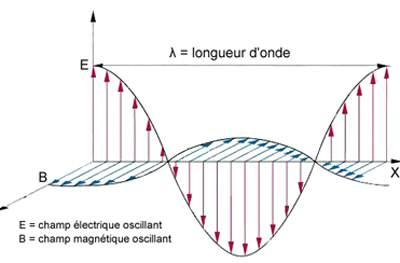
\includegraphics[scale=0.5]{21bbb8c912fd1c0c4853fcb9d75a3b7c.jpg}
\end{frame}
\begin{frame}{Propagation du signal en fonction du temps}

\end{frame}
\begin{frame}{caractéristiques des ondes}
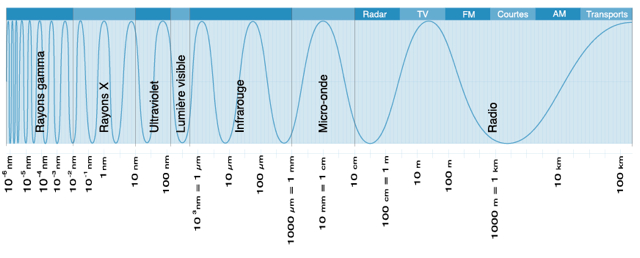
\includegraphics[scale=0.4]{a3400_electromagnatique_fr_g.jpg}
$$\lambda = \frac{c}{f}$$
$$ k=\frac{2 \pi}{\lambda}$$
\end{frame}
\end{document}